\mysection{Méthodologie}
Cette section a comme but expliquer les méthodes utilisées pour faire chaque tâche des parties 2 a 4 du travail, décrits dans les sections \ref{Deuxième Partie - Mise en Main} a \ref{Quatrième Partie - Intégration}.

\newcommand{\powerfactory}{DIgSILENT PowerFactory}
\mysubsection{Deuxième Partie - Mise en Main}
Comme dit, le logiciel \powerfactory a été utilisé pour faire des simulations du réseau, donc une petit explication du réseau e du logiciel sera fait dans cette section.

\mysubsubsection{À propos du \powerfactory}
Le \powerfactory est un logiciel beaucoup utilisé dans le métier d'Énergie, par entreprises comme \gls{EDF}, \gls{Enedis} pour faire des simulations des réseau électriques, que les permettent de vérifier stabilité en cas de panne et surcharge ou sous-charge de parties du réseau, calculer coûts d'opération et même programmer autres changements futur du réseau. Quelques autres instituts comme L'\gls{IETR} et \gls{Polimi}, par exemple l'utilise pour ses thèmes des thèses et autres recherches.   

\begin{figure}[H]
	\begin{center}	
		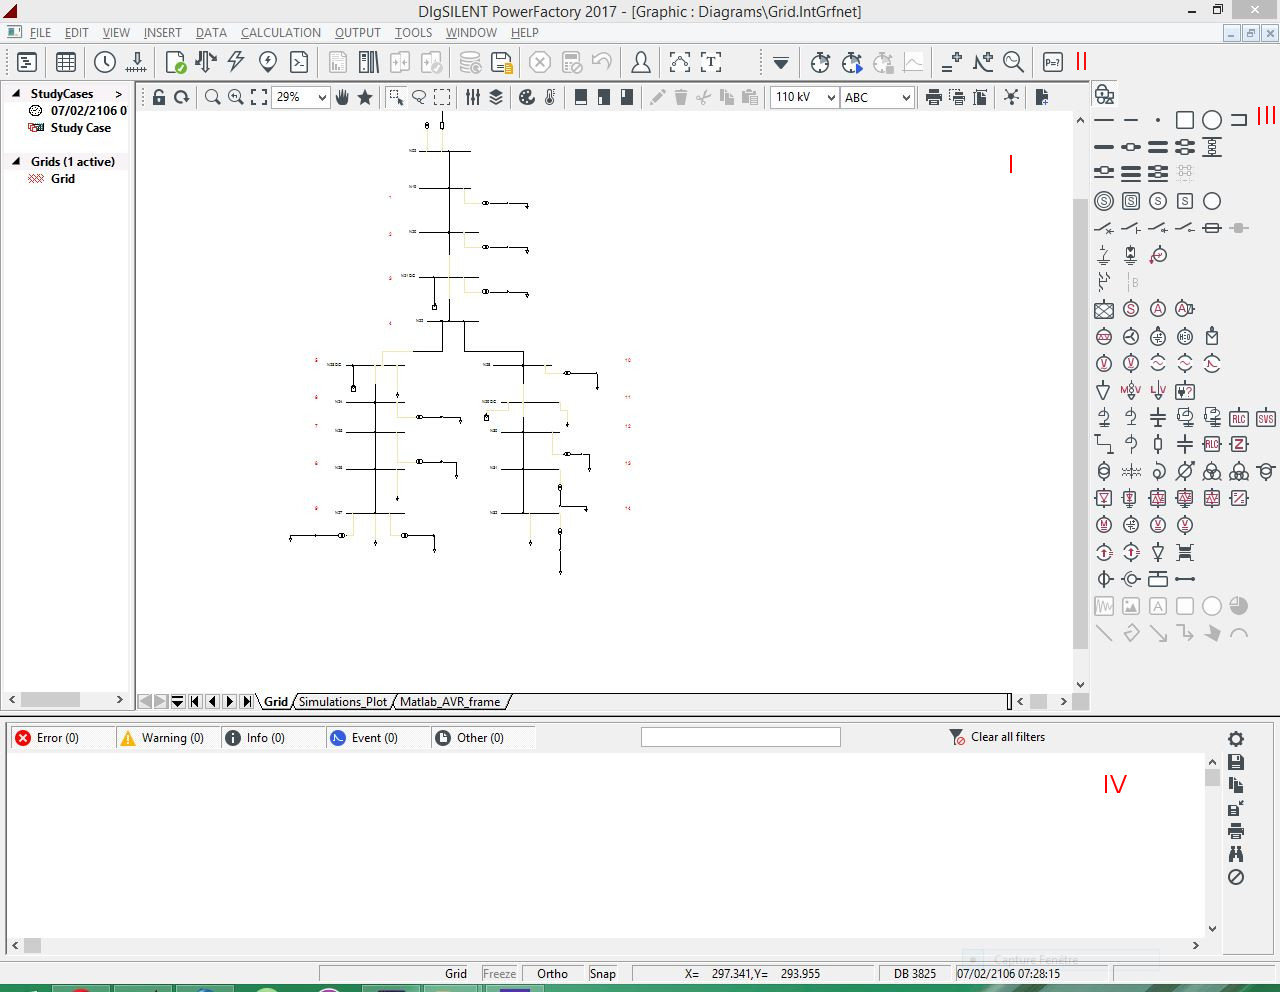
\includegraphics[width=\textwidth]{Methodologie/partie_2/gui_powerfactory_num.JPG}
		\caption{\gls{GUI} du \powerfactory.}
		\label{fig:gui_powerfactory}
	\end{center}
\end{figure}

\pagebreak
En peut voir dans la figure \ref{fig:gui_powerfactory} quelques panneaux basiques importants du \gls{GUI} du \powerfactory

\begin{enumerate}[I]
	\item Panneau Graphique\\ Où les diagrammes sont affichés, tant réseaux quant graphiques.
	\item Panneau des Outil\\ Où sont concentrés les outils du programme, pour modifier l'affichage, donnant une couleur différente par chaque bus par exemple; faire des diverses types de simulation,  de Court-circuit, calculs de flux de charge simulation \gls{RMS} et \gls{EMT}, etc.
	\item Panneau de Dessin\\ Outils pour dessiner des éléments du réseau, comme bus, transformateur, charge etc
	\item Panneau de Sortie\\ Où sont montrés les résultats des calculs et simulations, les avertissement et les erreurs.
\end{enumerate}


\mysubsection{À propos du réseau}
\newcommand{\trafoi}{40 MVA132/20}
\newcommand{\trafoii}{0.25MVA 20kV/0.4}
\newcommand{\trafoiii}{0.4MVA 20kV/0.4}
\newcommand{\trafoiv}{0.63MVA 20kV/0.4}
\newcommand{\cablei}{ARG7H1RX 185mmq}
\newcommand{\cableii}{ARG7H1RX 70mmq}
\newcommand{\cableiii}{Aerea Cu 70mmq}
Comme était dit, la figure \ref{fig:Diagramme_du_reseaux} démontre le réseau utilisé. Si on compare avec le réseaux utilisé en \cite{cosson:tel-01374469} et \cite{mariani2013controllo}, il est possible de voir que le réseaux de la figure  \ref{fig:Diagramme_du_reseaux} représente juste la moitié du original. Cette choix de prendre une partie du réseaux a comme raison la diminution des éléments et conséquemment la complexité des résolutions des simulations.

Le réseau est formé pour 16 charges et 3 générateurs distribués, 12 transformateurs.
Dans le réseau original deux des trois générateurs étaient des machines synchrones mais elles ont été remplacé par des panneaux photovoltaïque, a fin de faire les réponses des tests plus vite, en vue de la dynamique des panneaux considérablement plus vite que des machines synchrones, qui dépendent des constants électromécanique. 

A fin de faire une meilleur description du réseaux les tableaux \ref{tab:generateurs_du_reseaux} à \ref{tab:Charges} ont les caractéristiques des éléments qui la composent.

\hspace{-1.7cm}
\begin{minipage}{.5\textwidth}
\begin{table}[H]
	\captionsetup{justification=centering,margin=1cm}
	\caption{Générateurs Distribués du Réseau.}
	\label{tab:generateurs_du_reseaux}
	\centering
	\begin{tabular}{m{1cm}m{1.5cm}m{1.5cm}}
		\hline
		GD&P[MW] nominal&P[MW] 1p.m.\\
		\hline\\
		GD4&3.2&2.056124\\
		GD5&5.5&4.94595\\
		GD6&5.5&3.245381\\
		\hline\\
	\end{tabular}
\end{table}	
\end{minipage}
\begin{minipage}{.5\textwidth}
\begin{table}[H]
	\captionsetup{justification=centering}
	\caption{Transformateurs HV/MV.}
	\label{tab:Transformateurs_HV/MV}
	\centering
	\begin{tabular}{lc}
		\hline
		Model&40 MVA132/20\\
		\hline\\
		Puissance&50MVA\\
		Pertes Cuivre&176kW\\
		Tension de court-circuit Relative&15.5\%\\
		Taps&12\\
		Tension per Tap&1.5\%\\
		\hline\\
	\end{tabular}
\end{table}	
\end{minipage}
\begin{table}[H]
	\captionsetup{justification=centering,margin=2cm}
	\caption{Transformateurs MV/LV.}
	\label{tab:Transformateurs_MV/LV}
	\centering
	\begin{tabular}{lm{2cm}m{2cm}m{2cm}}
		\hline
		Modèle&0.25MVA 20kV/0.4&0.4MVA 20kV/0.4&0.63MVA 20kV/0.4\\
		\hline\\
		Puissance&250kVA&400kVA&630kVA\\
		Pertes Cuivre&2.6kW&3.7 kW&5.6kW\\
		Tension de court-circuit Relative&4\%&4\%&4\%\\
		Nombres de Transformateurs&1&6&4\\
		\hline\\
	\end{tabular}
\end{table}	
\vspace{-.5cm}
\begin{table}[H]
	\captionsetup{justification=centering,margin=2cm}
	\caption{Transformateurs.}
	\label{tab:Transformateurs}
	\centering
	\begin{tabular}{cc}
		\hline
		Nom&Modèle\\
		\hline\\
		TR AT/MT&\trafoi\\
		TR 2.19&\trafoiv\\
		TR 2.20&\trafoiii\\
		TR 2.21&\trafoiii\\
		TR 2.24&\trafoiii\\
		TR 2.25&\trafoiii\\
		TR 2.27.1&\trafoiv\\
		TR 2.27.3&\trafoiv\\
		TR 2.28&\trafoii\\
		TR 2.30&\trafoiv\\
		TR 2.31&\trafoiii\\
		TR 2.32&\trafoiii\\
		\hline\\
	\end{tabular}
\end{table}	
\vspace{-.5cm}
\begin{table}[H]
	\captionsetup{justification=centering,margin=2cm}
	\caption{Caractéristiques des Lignes.}
	\label{tab:Caractéristiques_des_Lignes}
	\centering
	\begin{tabular}{ccc}
		\hline
		Nom&Genre&Longueur[$ km $]\\
		\hline\\
		D2-02\_19&\cablei&3.6\\
		D2-19\_20	&\cablei&3.304\\
		D2-20\_21	&\cableiii&2.4\\
		D2-21\_22	&\cableiii&3.6\\
		D2-22\_23	&\cableiii&3\\
		D2-22\_28	&\cableii&2.4\\
		D2-23\_24	&\cableiii&3.08\\
		D2-24\_25	&\cableiii&1.65\\
		D2-25\_26	&\cableiii&1.8\\
		D2-26\_27	&\cableiii&2.2\\
		D2-28\_29	&\cableii&2.2\\
		D2-29\_30	&\cableii&2.4\\
		D2-30\_31	&\cableii&2.6\\
		D2-31\_32	&\cableii&2.7\\
		\hline\\
	\end{tabular}
\end{table}
\vspace{-.5cm}
\begin{table}[H]
	\captionsetup{justification=centering,margin=2cm}
	\caption{Lignes.}
	\label{tab:Lignes}
	\centering
	\begin{tabular}{llccccc}
		\hline
		Nom&Genre&Section[$ mm^2 $]&R[$ \Omega/km $]&L[$ mH/km $]&C[$ \mu F/km $]\\
		\hline\\
		\cablei&Câble&185&0.2180&0.350&0.2900\\
		\cableii&Câble&70&0.5800&0.41&0.2100\\
		\cableiii&Aérien&70&0.2681&1.286&0.0090\\
		\hline\\
	\end{tabular}
\end{table}	
\pagebreak
\begin{table}[H]
	\captionsetup{justification=centering,margin=2cm}
	\caption{Charges.}
	\label{tab:Charges}
	\centering
	\begin{tabular}{cccc}
		\hline
		Nom&Genre&P[$ MW $]1p.m.&Q[$MVAR$]1p.m.\\
		\hline\\
		C 2-19 &LV&0.1894&0.1265088\\
		C 2-20 &LV&0.1147&0.0774413\\
		C 2-21 &LV&0.1155&0.0782289\\
		C 2-23&MV&0&0.1\\
		C 2-24 &LV&0.1094&0.0741473\\
		C 2-25 &LV&0.1450&0.0984401\\
		C 2-26&MV&0.3993&0.2049369\\
		C 2-27.1&LV&0.2471&0.1656134\\
		C 2-27.2& MV&.6083&0.2971269\\
		C 2-27.3& LV&0.2094&0.1407233\\
		C 2-28 &LV&0.1205&0.08741\\
		C 2-29 &MV&0.1561&0.0798601\\
		C 2-30 &LV&0.1934&0.1347733\\
		C 2-31 &LV&0.0934&0.0640347\\
		C 2-32.1 &LV&0.1333&0.0923274\\
		C 2-32.2 &MV&0.5634&0.2791258\\
		\hline\\
	\end{tabular}
\end{table}	

\mysubsection{Troisième Partie - Programmation}

Pendant ce partie diverses scripts ont été crées en utilisant les langages MATLAB et Python, en intégration des bibliothèques Python du \powerfactory, qui pourvoit quelques fonctions pour accéder aux éléments du réseau, changer ses caractéristiques et faire des mesures de courant, tension etc.

Dans cette section chaque script est décrit par son fonctionnement, pour une description minutieuse, les codes sont présents dans l'appendice \ref{Programmes}. En ayant en tête que toutes fichiers utilisés sont disponibles dans le site \url{https://github.com/Accacio/scripts_powerfactory}.



\begin{enumerate}[\bfseries 4.3.1]
	\item $\mathbf{gain\_calc-load2bus.py}$\\
	\\Ce script change les valeurs de puissance réactive demandé par les charges pendant un intervalle de temps et prend les valeurs de tension du bus auquel la charge est connecté pendant ce temps et calcule le gain entre chaque charge et bus, formant une matrice de dimension $ 16\times16 $, avec le format suivant:
	\\	\begin{table}[H]\tiny
		\captionsetup{justification=centering,margin=0cm}
		\caption{Matrice des Gain de sortie du script $gain\_calc-load2bus.py$.}
		\centering
		\resizebox{\textwidth}{!}{\begin{tabular}{cccccc}
				$\frac{V_{N01}}{Q_{C 2-19}}$& $\frac{V_{N02}}{Q_{C 2-19}}$& $\frac{V_{N19}}{Q_{C 2-19}}$& $\frac{V_{N20}}{Q_{C 2-19}}$&$ \cdots $&$\frac{V_{N32}}{Q_{C 2-19}}$\\
				&&&&&\\
				$ \vdots $&$ \vdots $&$ \vdots $&$ \vdots $&$ \ddots $&$ \vdots $\\
%				$\frac{V_{N01}}{Q_{C 2-20}}$& $\frac{V_{N02}}{Q_{C 2-20}}$& $\frac{V_{N19}}{Q_{C 2-20}}$& $\frac{V_{N20}}{Q_{C 2-20}}$&$\cdots$&$\frac{V_{N32}}{Q_{C 2-20}}$\\
%				&&&&&\\
%				$\frac{V_{N01}}{Q_{C 2-21}}$& $\frac{V_{N02}}{Q_{C 2-21}}$& $\frac{V_{N19}}{Q_{C 2-21}}$& $\frac{V_{N20}}{Q_{C 2-21}}$&$\cdots$&$\frac{V_{N32}}{Q_{C 2-21}}$\\
%				&&&&&\\
%				$\frac{V_{N01}}{Q_{C 2-22}}$& $\frac{V_{N02}}{Q_{C 2-22}}$& $\frac{V_{N19}}{Q_{C 2-22}}$& $\frac{V_{N20}}{Q_{C 2-22}}$&$\cdots$&$\frac{V_{N32}}{Q_{C 2-22}}$\\
%				&&&&&\\
%				$\frac{V_{N01}}{Q_{C 2-24}}$& $\frac{V_{N02}}{Q_{C 2-24}}$& $\frac{V_{N19}}{Q_{C 2-24}}$& $\frac{V_{N20}}{Q_{C 2-24}}$&$\cdots$&$\frac{V_{N32}}{Q_{C 2-24}}$\\
%				&&&&&\\
%				$\frac{V_{N01}}{Q_{C 2-25}}$& $\frac{V_{N02}}{Q_{C 2-25}}$& $\frac{V_{N19}}{Q_{C 2-25}}$& $\frac{V_{N20}}{Q_{C 2-25}}$&$\cdots$&$\frac{V_{N32}}{Q_{C 2-25}}$\\
%				&&&&&\\
%				$\frac{V_{N01}}{Q_{C 2-26}}$& $\frac{V_{N02}}{Q_{C 2-26}}$& $\frac{V_{N19}}{Q_{C 2-26}}$& $\frac{V_{N20}}{Q_{C 2-26}}$&$\cdots$&$\frac{V_{N32}}{Q_{C 2-26}}$\\
				&&&&&\\
				$\frac{V_{N01}}{Q_{C 2-27.1}}$& $\frac{V_{N02}}{Q_{C 2-27.1}}$& $\frac{V_{N19}}{Q_{C 2-27.1}}$& $\frac{V_{N20}}{Q_{C 2-27.1}}$&$ \cdots $&$\frac{V_{N32}}{Q_{C 2-27.1}}$\\
				&&&&&\\
				$\frac{V_{N01}}{Q_{C 2-27.2}}$& $\frac{V_{N02}}{Q_{C 2-27.2}}$& $\frac{V_{N19}}{Q_{C 2-27.2}}$& $\frac{V_{N20}}{Q_{C 2-27.2}}$&$ \cdots $&$\frac{V_{N32}}{Q_{C 2-27.2}}$\\
				&&&&&\\				
				$\frac{V_{N01}}{Q_{C 2-27.3}}$& $\frac{V_{N02}}{Q_{C 2-27.3}}$& $\frac{V_{N19}}{Q_{C 2-27.3}}$& $\frac{V_{N20}}{Q_{C 2-27.3}}$&$ \cdots$&$\frac{V_{N32}}{Q_{C 2-27.3}}$\\
				&&&&&\\
				$\frac{V_{N01}}{Q_{C 2-28}}$& $\frac{V_{N02}}{Q_{C 2-28}}$& $\frac{V_{N19}}{Q_{C 2-28}}$& $\frac{V_{N20}}{Q_{C 2-28}}$&$\cdots$&$\frac{V_{N32}}{Q_{C 2-28}}$\\
				&&&&&\\
%				$\frac{V_{N01}}{Q_{C 2-29}}$& $\frac{V_{N02}}{Q_{C 2-29}}$& $\frac{V_{N19}}{Q_{C 2-29}}$& $\frac{V_{N20}}{Q_{C 2-29}}$&$\cdots$&$\frac{V_{N32}}{Q_{C 2-29}}$\\
%				&&&&&\\
%				$\frac{V_{N01}}{Q_{C 2-30}}$& $\frac{V_{N02}}{Q_{C 2-30}}$& $\frac{V_{N19}}{Q_{C 2-30}}$& $\frac{V_{N20}}{Q_{C 2-30}}$&$\cdots$&$\frac{V_{N32}}{Q_{C 2-30}}$\\
%				&&&&&\\
%				$\frac{V_{N01}}{Q_{C 2-31}}$& $\frac{V_{N02}}{Q_{C 2-31}}$& $\frac{V_{N19}}{Q_{C 2-31}}$& $\frac{V_{N20}}{Q_{C 2-31}}$&$\cdots$&$\frac{V_{N32}}{Q_{C 2-31}}$\\
%				&&&&&\\
				$ \vdots $&$ \vdots $&$ \vdots $&$ \vdots $&$ \ddots $&$ \vdots $\\
				&&&&&\\
				$\frac{V_{N01}}{Q_{C 2-32.1}}$& $\frac{V_{N02}}{Q_{C 2-32.1}}$& $\frac{V_{N19}}{Q_{C 2-32.1}}$& $\frac{V_{N20}}{Q_{C 2-32.1}}$&$\cdots$&$\frac{V_{N32}}{Q_{C 2-32.1}}$\\
				&&&&&\\
				$\frac{V_{N01}}{Q_{C 2-32.2}}$& $\frac{V_{N02}}{Q_{C 2-32.2}}$& $\frac{V_{N19}}{Q_{C 2-32.2}}$& $\frac{V_{N20}}{Q_{C 2-32.2}}$&$\cdots$&$\frac{V_{N32}}{Q_{C 2-32.2}}$\\
		\end{tabular}}		
	\end{table}
	Où \gls{Vnxx}  et \gls{Qcxx} sont la tension du bus $ Nxx $ e la puissance réactive de la charge $ Cx-xx $.
	
	\item $\mathbf{gain\_calc-generator2bus-test\_1.py}$\\
	\\Ce Script change les valeurs de puissance réactive des générateurs pendant un intervalle de temps e prends les valeurs de tension du bus auquel le générateur est connecté pendant ce temps et calcule le gain entre chaque générateur et bus, formant une matrice de dimension $ 3\times3 $. L'allure de la courbe utilisé peut être vu dans la figure \ref{fig:gaincalcgenerator2bustest1}. Le format de la matric est montré dans letableau \ref{tab:gaincalcgenerator2bustest1}.
	\begin{figure}[H]
		\begin{center}	
			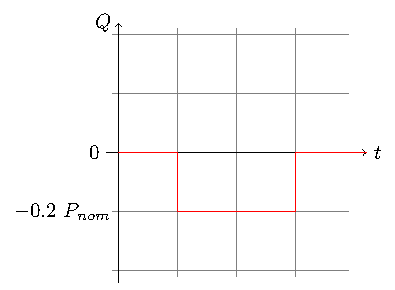
\includegraphics[width=8cm]{Methodologie/partie_3/gain_calc-generator2bus-test_1.pdf}
			\caption{Allure de la courbe utilisé pendant le Test 1.}
			\label{fig:gaincalcgenerator2bustest1}
		\end{center}
	\end{figure}
\begin{table}[H]
	\captionsetup{justification=centering,margin=2cm}
	\caption{Matrice des Gain de sortie du script $gain\_calc-generator2bus-test\_1.py$.}
	\label{tab:gaincalcgenerator2bustest1}
	\centering
	\begin{tabular}{ccc}
		$ \frac{V_{N21}}{Q_{GD4}} $&$ \frac{V_{N29}}{Q_{GD4}} $&$ \frac{V_{N23}}{Q_{GD4}} $\\
		&&\\
		$ \frac{V_{N21}}{Q_{GD5}} $&$ \frac{V_{N29}}{Q_{GD5}} $&$ \frac{V_{N23}}{Q_{GD5}} $\\
		&&\\
		$ \frac{V_{N21}}{Q_{GD6}} $&$ \frac{V_{N29}}{Q_{GD6}} $&$ \frac{V_{N23}}{Q_{GD6}} $\\
	\end{tabular}
\end{table}
Où \gls{Qgdx} est la puissance réactive du générateur $ GDx $.

	\item $\mathbf{gain\_calc-generator2bus-test\_2.py}$\\
	\\Fondamentalement le même que $gain\_calc-generator2bus-test\_1.py$, mais la courbe de changement de puissance suivre l'allure de la figure \ref{fig:gaincalcgenerator2bustest2}. Le format de la matrice est le même montré dans letableau \ref{tab:gaincalcgenerator2bustest1}.
	\begin{figure}[H]
		\begin{center}	
			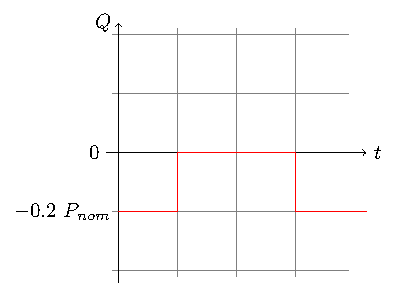
\includegraphics[width=8cm]{Methodologie/partie_3/gain_calc-generator2bus-test_2.pdf}
			\caption{Allure de la courbe utilisé pendant le Test 2.}
			\label{fig:gaincalcgenerator2bustest2}
		\end{center}
	\end{figure}
	\item $\mathbf{import\_generator\_csv.py}$\\
	\\Ce script prend des fichiers \gls{CSV} qui a données de puissance nominal, active et réactive des générateurs, et les charge en chaque générateur.
	\begin{figure}[H]
		\begin{center}	
			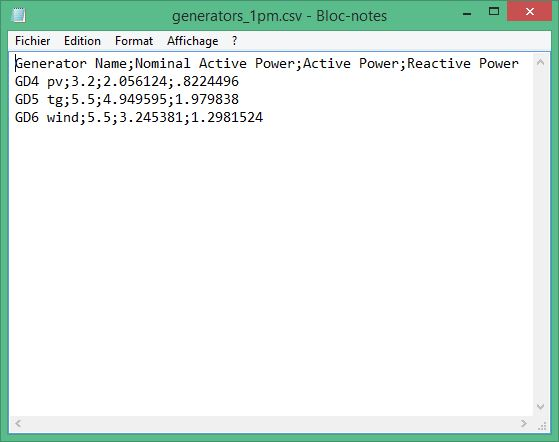
\includegraphics[width=8cm]{Methodologie/partie_3/csv_sample.JPG}
			\caption{Exemple d'un fichier CSV, séparé par point-virgule.}
			\label{fig:csv_sample}
		\end{center}
	\end{figure}
	La choix d'utiliser fichiers \gls{CSV} a été fait en raison de ce type de fichier est texte sans brut sans formatage, sa taille est très réduite. Et ce type de fichier est très simple pour faire des modifications et création a partir d'untableau \verb|.xls|, ainsi que la conversion entre ces deux extensions.  
	\\
	\item $\mathbf{import\_load\_csv.py}$\\
	\\Ce script prend des fichiers \gls{CSV} qui a données de puissance active et réactive des charges, et les charge en chaque respective charge.
	\\
	\item $\mathbf{csv2mat.m}$\\
	\\Ce script fait en MATLAB prend un fichier \gls{CSV} sorti d'une simulation du \powerfactory et le transforme en un fichier .mat. Il crée une structure composés par autres structures qui sont les éléments du circuit et composées par ses données  pendant le temps, a fin de les utiliser pour faire des graphiques.
	\\
	\item $\mathbf{printpdf.m}$\\
	\\Ce script a été créé pour faire les plots des graphiques et les sauvegarder en fichier \verb|.pdf| pour un futur use dans les rapports (ce rapport par exemple). 
	\\
	\item $\mathbf{teste\_simul.py}$\\
	\\Ce script crée un événement des changement de valeur de puissance active de la charge C 2-29 MT ind en augmentant sa valeur en 100\% par un période de temps et après prend les valeurs de puissance active et réactive des cette même charge et la tension des bus N21 N23 et N29 ( où les générateurs sont connectés ) pendant le temps de la simulation et en exportant en un fichier $ \verb|.csv| $.
	\\ 
\end{enumerate}

\mysubsection{Quatrième Partie - Intégration}
Le but de cette partie était reproduire les simulations du réseau (figure \ref{fig:Diagramme_du_reseaux}) en utilisant le régulateur vu en \cite{cosson:tel-01374469}, montré dans la figure \ref{fig:regulateur}.

\begin{figure}[H]
	\centering
	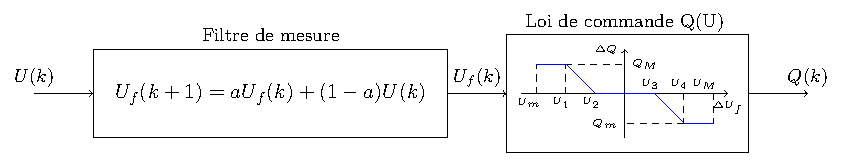
\includegraphics[]{Figuras/Methodologie/partie_4/regulateur}
	\caption{Diagramme représentative du régulateur.}
	\label{fig:regulateur}
\end{figure}

Les valeurs utilisés pour la loi de commande sont dans le tableau suivante:
\begin{table}[H]
	\captionsetup{justification=centering,margin=0cm}
\caption{Matrice des Gain de sortie du script}
\centering
\label{tab:valeurs_loicommande}
\begin{tabular}{|c|c|}
	\hline
Variable&Valeur\\
	\hline
$ U_m $&18 $kV$\\
	\hline
$ U_1 $&19 $kV$\\
	\hline
$ U_2 $&19,25 $kV$\\
	\hline
$ U_3 $&20,75 $kV$\\
	\hline
$ U_4 $&21 $kV$\\
	\hline
$ U_M $&21 $kV$\\
	\hline
$ Q_m $&-0,4 $ P_max $\\
	\hline
$ Q_M $&0,4 $ P_max $\\
	\hline
\end{tabular}
\end{table}


Pour construire le modèle du régulateur dans le \powerfactory, il y a deux façons, faire toute la construction dedans PowerFactory en usilisant sa langage propriétaire de description des systèmes, \gls{DSL},  ou faire une intégration avec MATLAB et utiliser les outils des \textit{ToolBox} déjà créés.

A fin de faire l'intégration entre MATLAB et \powerfactory, au minimum deux choses sont nécessaires :
\begin{enumerate}
	\item Un Bloc générique défini au PowerFactory qui fait l'appel a un fichier \verb|.m|
	\item Un fichier \verb|.m| qui décrit le fonctionnement du bloc
	
\end{enumerate}

Comme ont voulait faire un régulateur dans le Simulink, un autre fichier, \verb|.mdl|, était nécessaire. Ce fichier est appelé par le fichier \verb|.m| et le donne les sorties de simulation.

La période d'échantillonnage du filtre númerique est de $ 1s $ et le pas de la simulation au PowerFactory est de $ 10ms $. Comme une façon de régler la fréquence d'appel au MATLAB n'était pas trouvé, la solution plus simple était l'implémentation du filtre dehors le MATLAB, donc un échantillonneur e le propre filtre ont était construits dans l'interface du PowerFactory, comme un peut voir dans les figures \ref{fig:DIgSILENT_Matlab_AVR_frame} a \ref{fig:DIgSILENT_Matlab_AVR_frame_matlab} et dans le simulink la loi de commande \ref{fig:simulink}.

\begin{minipage}{\textwidth}
	\centering
\begin{minipage}{.475\textwidth}
	\begin{figure}[H]
		\captionsetup{justification=centering,margin=0cm}
		\begin{center}	
			\includegraphics[width=\textwidth]{"./Methodologie/partie_4/DIgSILENT_Matlab_AVR_frame"}
			\caption{Diagramme du régulateur \\assemblé dans PowerFactory.}
			\label{fig:DIgSILENT_Matlab_AVR_frame}
		\end{center}
	\end{figure}
\end{minipage}
\begin{minipage}{.475\textwidth}
	\begin{figure}[H]
		\captionsetup{justification=centering,margin=0cm}
		\begin{center}	
			\includegraphics[width=\textwidth]{"./Methodologie/partie_4/DIgSILENT_Matlab_AVR_frame_filtre"}
			\caption{Filtre et Échantillonneur implémentées dans PowerFactory.}
			\label{fig:DIgSILENT_Matlab_AVR_frame_filtre}
		\end{center}
	\end{figure}
\end{minipage}\\
\begin{minipage}{.475\textwidth}
\begin{figure}[H]
	\captionsetup{justification=centering,margin=0cm}
	\begin{center}	
		\includegraphics[width=\textwidth]{"./Methodologie/partie_4/DIgSILENT_Matlab_AVR_frame_matlab"}
		\caption{Bloc Générique Matlab.}
		\label{fig:DIgSILENT_Matlab_AVR_frame_matlab}
	\end{center}
\end{figure}
\end{minipage}
\begin{minipage}{.475\textwidth}
\begin{figure}[H]
	\captionsetup{justification=centering,margin=0cm}
	\begin{center}	
		\includegraphics[width=\textwidth]{"./Methodologie/partie_4/simulink"}
		\caption{Loi de commande en Simulink.}
		\label{fig:simulink}
	\end{center}
\end{figure}
\end{minipage}
\end{minipage}

Le diagramme du modèle est dans la figure \ref{fig:DIgSILENT_Matlab_AVR_frame_withoutmatlab}, et comme on peut voir, c'est  essentiellement la même chose, le code dedans le bloc générique qui a été changé. 

Les codes utilisés pour les modèles pourront être trouvé dans \todo{APENDICE DE CODIGO}

\begin{figure}[H]
	\begin{center}	
		\includegraphics[width=.475\textwidth]{"./Methodologie/partie_4/DIgSILENT_Matlab_AVR_frame_withoutmatlab"}
		\caption{Régulateur fait seulement en PowerFactory.}
		\label{fig:DIgSILENT_Matlab_AVR_frame_withoutmatlab}
	\end{center}
\end{figure}

\mysubsubsection{À propos des temps de simulation}
Après faites toutes connexions et quelques tests avec le régulateur, ont a vu qu'une simulation de $ 50s $ a duré approximativement $ 5min $. Donc deux autres modèles ont été créés a fin de comparaison. Un avec toute le régulateur dans le PowerFactory et un autre avec la loi de commande fait dans le MATLAB ( le seule changement était le code \verb|.m|). Avec ces deux modèles une simulation de $50s$ a duré approximativement $ 50s $.
On peut voir dans le tableau \ref{tab:comparaisontempssimul} la comparaison entre les temps de simulation:

\begin{table}[H]
	\centering
	\captionsetup{justification=centering,margin=2cm}
	\caption{Temps réel de simulation en secondes\\ pour une simulation de $ 10s $}
	\label{tab:comparaisontempssimul}
	\begin{tabular}{lcc}
		&Cond. Ini.&Simulation\\
		Sans Contrôle&1&10\\
		Powerfactory&1&10\\
		Powerfactory$ \leftrightarrows $MATLAB&20&12\\
		Powerfactory$ \leftrightarrows $MATLAB$ \leftrightarrows $Simulink&57&140\\
	\end{tabular}
\end{table}
On peut vérifier que il ne vaut pas la peine utiliser le Simulink pour faire ce genre de simulation cas il soit appellé  a chaque $ 0.01s $. Nouveaux tests doivent être faits a fin de confirmer si même faisant appels a chaque seconde si les temps se maintiennent.



